\documentclass{article}

\usepackage[francais]{babel}
\usepackage[T1]{fontenc}
\usepackage{moreverb}       % verbatim with tab

\usepackage{wrapfig}
\usepackage{graphicx}
\usepackage{geometry}
\geometry{hmargin=2.5cm}
\usepackage{amsmath}
\usepackage{siunitx}

\usepackage{graphicx}
\usepackage{subcaption}
\usepackage{float}
\usepackage{hyperref}
\usepackage{setspace}
\usepackage{xcolor}
\usepackage{pdfpages}
\usepackage{enumitem}
\usepackage{lscape}

\usepackage{fancyhdr}       % en-têtes
\usepackage{lastpage}       % numéro de dernière page

\title{Systèmes logiques programmés\bigbreak \bigbreak
    \large Dossier récapitulatif\bigbreak
    \normalsize Programmation d'un générateur de signaux en assembleur sur PIC16F887\bigbreak}
\date{2020 -- 2021}
\author{Laura Binacchi}

\pagestyle{fancy}
\renewcommand\headrulewidth{1pt}
\fancyhead[L]{Laura Binacchi}
\fancyhead[C]{Systèmes logiques programmés}
\fancyhead[R]{\today}


\begin{document}
    \pagenumbering{gobble}
    
\includepdf[pages={1}]{pdg}
    \newpage
    \tableofcontents
    \newpage
    \pagenumbering{arabic}

    \section{Cahier des charges}
    \paragraph{}
    Sur base des modules élémentaires et exemples vus au cours (ports, interruptions, timers, CCP, SPI, I2C, ADC, LCD) développer sous MPLABX une application en langage d’assemblage sur PIC série 16F8xx ou 16F9xx ainsi que le modèle Proteus permettant de la simuler. L’application devra utiliser au moins une source d’interruptions, gérer un LCD et connecter au moins un circuit esclave en mode SPI ou I2C.

    \paragraph{}
    L’application permettra de générer un signal simple, carré ou triangulaire, de fréquence et rapport cyclique paramétrables. Le signal sera généré par l’intermédiaire d’un DAC 8 bits.

    \paragraph{}
    Les datasheets des PIC et des circuits nécessaires sont données, vous pouvez en choisir d’autres si vous le souhaitez et que cela se justifie. Vous ne devez évidemment pas utiliser tous les circuits, juste ceux nécessaires pour votre application. Une routine de conversion bianire / BCD est également donnée.

    \paragraph{}
    Les caractéristiques de l'applications sont données dans la liste ci-dessous. Vous avez le choix du dispositif de saisie (boutons, clavier, roue codeuse, dip switch, ...) et de la taille de l’écran, minimum 2x16 caractères. Vous pouvez faire plus que demandé, pas moins.
    \begin{itemize}[label=$\bullet$]
        \item Application : générateur de signaux
        \item PIC : 16F876A, 16F877A ou 16F887
        \item Bus : I2C
        \item Sortie signal : DAC 0808 connection directe au PIC
        \item Paramètres : fréquence, type et rapport cyclique du signal
        \item LCD : connection au bus I2C via IO expander 16 bits
    \end{itemize}


    \newpage
    \section{Analyse}
    \paragraph{}
    Le générateur de signaux est implémenté par le module de comparaison du microcontrôleur : une interruption est générée à un intervalle régulier pour mettre à jour la valeur du signal sur le convertisseur numérique analogique.

    \paragraph{}
    Les valeurs du signal sont stockées dans un vecteur de 100 bytes initialisé au démarrage de la génération de signal. A chaque itération de l'interruption déclenchée par le module CCP, la valeur du signal est récupérée et projetée sur le DAC. La gamme de PIC proposée ne disposant pas de banque assez grande pour stocker un vecteur de cette taille, le tableau de 100 valeurs représantant le signal est stocké dasn deux vecteurs de 50 bytes répartis sur les banques 2 et 3.

    \paragraph{}
    Le signal généré doit être paramétrable : il faut donc implémenter un mode de configuration. Celui-ci est totalement indépendant du mode de génération du signal : les deux modes de fonctionnement ne peuvent pas être concurrents car ils utilisent tous deux des interruptions et que la gamme de microcontrôleurs PIC16F ne permet pas de donner un niveau de priorité supérieur à une interruption sur l'autre. Les deux interruptions ne sont donc pas activées en même temps : le mode de génération du signal active l'interruption par le module CCP et désactive l'interruption sur la PIN RB0 et le mode de configuration fait l'inverse.
    
    \paragraph{}
    Un switch permet de choisir le mode de fonctionnement et une LED permet de le visualiser : elle est allumée lorsque le signal est généré et éteinte en mode de configuration.

    \paragraph{}
    Un écran LCD permet de visualiser les paramètres du signal : forme du signal, fréquence, rapport cyclique et amplitude. Le microcontrôleur communique avec le LCD via son bus I$^2$C par l'intermédiaire d'un I/O expander 16 bits (ce qui permet de configurer le LCD en mode 8bits).

    \paragraph{}
    Un ensemble de sept boutons permet de régler les paramètres du signal. Cet ensemble de boutons est lui aussi connecté au microcontrôleur via son bus I$^2$C et un I/O expander de 8 bits. L'I/O expander génère une interruption sur la PIN RB0 du microcontrôleur lorsqu'une entrée est détectée.

    \paragraph{}
    La sélection de la forme du signal se fait par un seul bouton qui permet de faire défiler la forme du signal : initialisé à carré, il passe ensuite à triangulaire, puis dent de scie, puis carré et ainsi de suite. Le signal en dent de scie est une forme particulière du signal triangulaire dont le rapport cyclique est égal à 0 ou à 100\%. Il aurait pu ne pas être répété : l'implémenter permet toutefois de sélectionner plus rapidement cette forme de signal plutôt qu'en paramétrant le rapport cyclique du signal triangulaire.

    \paragraph{}
    La fréquence peut être augmentée et diminuée par deux boutons différents. Elle est initialisée à \SI{1}{\kilo\hertz} et peut-être diminuée en augmentant la valeur du prescaler du timer qui génère l'interruption : elle sera donc divisée par deux pour atteindre une valeur minimum de \SI{125}{\hertz} (prescaler 1:8). La fréquence aurait également pu être diminuée en augmentant la valeur de comparaison du module CCP : le pas de diminution aurait alors pu être plus fin. La fréquence aurait également pu être réglée en diminuant le nombre de valeurs du tableau affichées : elle aurait été doublée en n'affichant qu'une valeur sur deux, etc. Le générateur aurait alors pu montrer à des fréquences plus élevées mais au prix d'un signal moins lisse.

    \paragraph{}
    La rapport cyclique est réglé par deux boutons. Il s'exprime en pourcentage et peut être diminué et augmenté par pas de 10\%. Ses valeurs sont comprises entre 0 et 100\% inclus.

    \paragraph{}
    L'amplitude du signal s'exprime elle aussi en pourcentage : il s'agit d'un poucentage de la tension de référence donnée au convertisseur numérique-analogique. L'amplitude varie comme le rapport cyclique entre 0 et 100\% par pas de 10 et est réglée par deux boutons.

    \paragraph{}
    Les différents réglages des paramètres nécessitent l'implémentation d'une arithmétique entière non signée sur 16 bits, e.g. pour diviser la fréquence par deux. L'affichage des paramètres nécessite quant à lui l'implémentation de routines de conversion des nombres binaires vers du BCD.


    \section{Choix du matériel}
    \paragraph{}
    Le développement du générateur de signaux périodique se base sur un hardware composé de :
    \begin{itemize}[label=$\bullet$]
        \item un microcontrôleur \textbf{PIC16F887};
        \item un \textbf{switch} connecté directement au microcontrôleur (PORTC, 0) permettant de sélectionner le mode de fonctionnement : génération de signal (switch fermé) ou configuration du signal (switch ouvert);
        \item une \textbf{LED} connectée directement au microcontrôleur (PORTC, 1) pour visualiser le mode de fonctionnement;
        \item un convertisseur numérique-analogique \textbf{DAC0808} connecté directement au port D du microcontrôleur;
        \item un écran LCD \textbf{LM044L} (de $4\times 20$ caractères) connecté via un I/O expander 16 bits \textbf{PCA9535} (bus I$^2$C) pour afficher les paramètres du signal;
        \item sept boutons connectés via un I/O expander 8 bits \textbf{PCA9554} (bus I$^2$C) pour paramétrer le signal.
    \end{itemize}

    \paragraph{}
    Parmi les microcontrôleur sproposés, j'ai choisi le PIC16F887. J'ai écarté le PIC16F876A car il n'est pas recommandé par \emph{Microchip} pour les nouveaux développements\footnote{Voir la mention \emph{Status: Not Recommended for new designs} affichéé sur site du fabricant \url{https://www.microchip.com/wwwproducts/en/PIC16F876A}}. Le PIC16F887 a plus de fonctionnalités que le PIC16F877A, e.g plus de PIN qui peuvent être configurées en analogique et un mode ECCP. Ces fonctionnalités ne sont pas utiles pour le générateur de signaux. J'ai tout de même choisi ce microcontrôleur car il est deux fois moins cher que le PIC16F877A\footnote{Prix de référence sur le site du fabricant : 2,60 euros pour le PIC16F887-I/P contre 4,56 euros pour le PIC16F877A-I/P et 4,39 euros pour le PIC16LF876A-I/SP.}.

    \paragraph{}
    Le DAC0808 est connecté directement au microcontrôleur et pas via bus de communication. C'est la manière la plus rapide de le connecter au microcontrôleur : la valeur est directement envoyée au DAC sans le temps supplémentaire nécessaire à l'envoi par un bus de communication (envoi des conditions de démarrage et de fin de communication, envoi de chaque bit les uns à la suite des autres, etc).

    \paragraph{}
    Le choix du mode de fonctionnement est fait par un switch plutôt que par un bouton car il n'y a que deux modes de fonctionnement : la valeur de la PIN à laquelle est connecté le switch peut donc être testée directement sans devoir garder en mémoire le mode choisi.

    \paragraph{}
    Le mode de fonctionnement est visualisé par une LED plutôt qu'affiché sur le LCD afin de ne garder le LCD que pour l'affichage des paramètres du signal.

    \paragraph{}
    J'ai choisi un LCD de 4 lignes (deux de plus que le minimum recommandé) pour pouvoir afficher un paramètre par ligne et donc privilégier la lisibilité des paramètres. Il est connecté au microcontrôleur via l'I/O expander recommandé dans les consignes pour la communication I$^2$C.

    \paragraph{}
    Les entrées sont elles aussi connectées via un I/O expander du même fabricant que l'I/O expander du LCD mais en 8 bits (suffisants pour connecter les 7 entrées). Les changements de paramètres pourront ainsi être détectés par interruption plutôt que par polling.


    \section{Projet Proteus}
    \paragraph{}
    Le projet Proteus est divisé en deux feuilles : la première présente les éléments avec lesquels l'utilisateur interagit et la seconde les éléments cachés.

    \paragraph{}
    La première feuille comprend les éléments de l'interface humain-machine :
    \begin{itemize}[label=$\bullet$]
        \item l'écran LCD;
        \item la LED de visualisation du mode de fonctionnement;
        \item les boutons et swith représentés par des états logiques pour simplifier le schéma;
        \item l'oscilloscope permettant de visualiser le signal de sortie du DAC.
    \end{itemize}

    \begin{figure}[H]
        \centering
        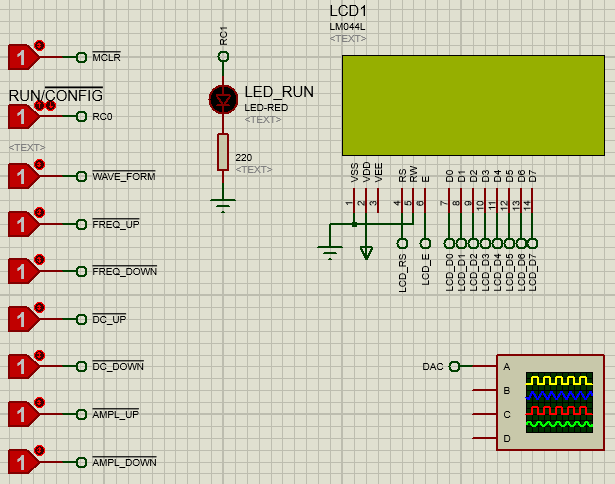
\includegraphics[width=.55\textwidth]{./images/proteus_rs1.png}
    \end{figure}

    \paragraph{}
    La seconde feuille comprend les éléments de hardware cachés :
    \begin{itemize}[label=$\bullet$]
        \item le microcontrôleur;
        \item les I/O expander PCA9535 et PCA9554 et les circuits associées (résistances de pull-up);
        \item le DAC et les circuits associés (résistances de pull-up et amplificateur opérationnel en buffer).
    \end{itemize}

    \begin{figure}[H]
        \centering
        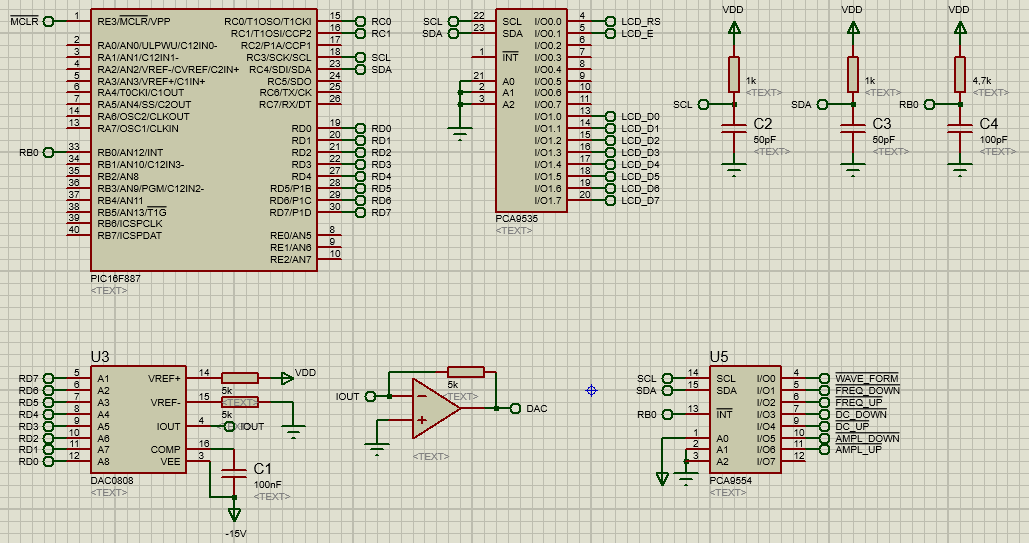
\includegraphics[width=\textwidth]{./images/proteus_rs2.png}
    \end{figure}

    \paragraph{}
    Les circuits associés aux différents éléments sont ceux fournis par leurs datasheets.



    \section{Configuration}
    \paragraph{}
    Pour compiler le projet avec MPLABX, les options suivantes doivent être ajoutées au linker pour définir l'emplacement des vecteurs de reset et d'interruption : \texttt{-presetVec=0x00} et \texttt{-pinterVec=0x04}.

    \paragraph{}



    \paragraph{}
    Le PIC est configuré dans le programme principal 

    ; init parameters
    ; compute the frequency
    INIT16	OPL16, 5000
    MOV16	OPR16, CCPR2L
    call	DIV16
    MOV16	frequency, RESULT32

    beaucoup de calls -> facilite la lecture et la compréhension du code mais ralenti l'initialisation (1 call = 4 Tcy)


    configuration de ce qui est en entrée et de ce qui est en sortie dans la fonction ini io
    configuration des entrées / sorties
    entrées : switch du mode
    sorties : LED de mode, DAC et bus I2C

    configuration des interruptions : options du linker
    interruption en RB0 (déclenchée sur front descendant car à 1 au repos/ en logique inverse) -> configuré en entrée + en digital car par défaut analogique
    interruption par module CCP2 (pas le 1 car ECCP) -> timer1, prescaler...
    wadchdog timer si bouton de mode appuyé trop longtemps (je pense que c'est le seul qui peut poser problème mais pas sûr)

    configuration du I2C + des PCA (en entrée et en sortie) + du LCD
     


    \section{Fonctionnement du programme}
    \subsection{Configuration du signal}

    \paragraph{}
    Initialisation : désactivation des interruptions, remise à 0 du DAC


    \subsection{Génération du signal}


    signal carré utilise le tableau de valeur aussi -> possibilité de régler le duty cycle au pourcent près pour un tableau de 100 valeurs


    \subsection{Conversions en caractères ASCII}
    \paragraph{}
    Les conversions des nombres en caractères ASCII sont définies dans le fichier \emph{16bits\_bin\_bcd\_ascii.inc} et implémentées dans le fichier \emph{16bits\_bin\_bcd\_ascii.s}. Elles permettent de convertir un nombre binaire en caractères ASCII ou de le transformer en BCD pour permettre un affichage en décimal. L'affichage décimal peut se faire pour un nombre de 8 ou de 16 bits et peut donc afficher une valeurs jusqu'à 65535 (\texttt{0xFFFF}).

    \subsection{Arithmétique 16 bits}
    \paragraph{}
    J'ai repris les opérations d'arithmétique 16 bits vues au cours et la séparation des fichiers contenant les macros (\emph{16\_bits\_arithmetic\_macros.inc}), les définitions des fonctions (\emph{16\_bits\_arithmetic.inc}) et l'implémentation des fonctions (\emph{16\_bits\_arithmetic.s}).

    \paragraph{}
    J'ai ajouté la fonction \texttt{MUL8} qui permet de multiplier deux nombres de 8 bits et d'obtenir un résultats de 16 bits. J'ai également ajouté le test de la valeur \texttt{0} pour le dividende de la division 16 bits.

    \paragraph{}
    Toutes les macros et fonctions ne sont pas utilisées mais elles sont laissées dans les fichiers pour pouvoir réutiliser ceux-ci dans d'autres projets.



    \section{Les tests réalisés}
    \paragraph{}
    J'ai testé le paramétrage du signal dans Proteus en faisant passer les paramètres par toutes les valeurs possibles et en vérifiant que les affichages correspondent bien aux changements attendus. Ce test m'a permis de vérifier que le programme ne permette pas de dépasser les valeurs limites des paramètres : 0 et 100 pour le rapport cyclique et l'amplitude et 125 et 1000 pour la fréquence.

    \paragraph{}
    L'adéquation entre les paramètres du signal et le signal produi est vérifiée par l'observation du signal à l'oscilloscope : elle permet de vérifier la forme du signal, sa fréquence, son rapport cyclique et son amplitude assez facilement avec les paramètres possibles du signal.

    \paragraph{}
    Tout au long du développement, j'ai vérifié les valeurs contenues dans les différents registres du PIC grâce à l'outil \emph{Watch Window} des options de debug de Proteus. J'ai également vérifié régulièrement les valeurs des PIN en les connectant à l'oscilloscope. Par exemple, pour mettre en place la communication du LCD via le bus I$^2$C, j'ai vérifié la valeur contenue dans le registre \texttt{SSPBUF} et j'ai vérifié les états des PIN SDA et SCL à l'oscilloscope.

    \paragraph{}
    A partir du moment où mon programme implémentait le LCD et où il est devenu trop complexe que pour retrouver facilement l'adresse d'une variable, j'ai utilisé le LCD et la conversion binaire vers ASCII pour vérifier les différentes valeurs intermédiaires des calculs de paramètres.



    \section{Les problèmes rencontrés}
    \paragraph{}

    configuration 
    
\end{document}